% Methodology
%
%	Experimental Set-up
%	Model Equations

\chapter{Methodology}

\section{Estimation of the amount of data}

Presently the \gls{LHC} is working with an interval of 50ns between 
\glspl{bunch} this correspond to a bunch every 10 \glspl{bucket}. But the 
\gls{OP} is planning to move to 25ns \glspl{bunch} spacing this would mean 
5 \glspl{bucket} between \glspl{bunch}. With the \gls{rffreq} we can compute 
the number of acquisitions per seconds.

$$for~50~ns~: \frac{400.789M}{20} = 20'039'450 \leq 2^{25}$$

$$for~25~ns~: \frac{400.789M}{10} = 40'078'900 \leq 2^{26}$$ 

This represent the amount of data for one pickup (\gls{BPM}), in the case of 
\gls{ADT} we have two of them per beam and per plane so as the \gls{LHC} has 
two rings and for each ring there are two transversal plane and there are 
two pickups per plane. This means we still have to multiply this value by 
eight.

$$for~50~ns~: 2^{25} * 8 = 2^{28}$$

$$for~25~ns~: 2^{26} * 8 = 2^{29}$$

As \glspl{FFT} on \glspl{GPU} start to be be faster than \glspl{CPU} around 
$2^{15}$ acquisitions it seems interesting to study this kind of system to 
compute the \gls{tune}.

\section{Measurement with the ADT}

In order to check the feasibility of the system and to have a good prototype
the first test will be to excite some of the \glspl{bunch} and acquire the
\gls{tune} using the \gls{ADT} during the end of 2012 run.

A piece of software has been developed that will acquire the bunch by bunch 
acquisition and compute various algorithm on the data using the \gls{CPU} 
and the \gls{FFTW} library in the \gls{CERN} infrastructure using \gls{CO} 
group control system and the \gls{OP} group infrastructure.

\section{Experimental Set-up}

Using the \gls{ADT} \glspl{BPM} we acquired data in the machine during 3 
independant \glspl{MD}. Most of the data taking was done in parallel to 
other normal LHC operation or during \gls{ADT} dedicated \gls{MD} time.

   \subsection{Hardware}

\begin{figure}
\caption{ADT acquisition hardware}
\centering
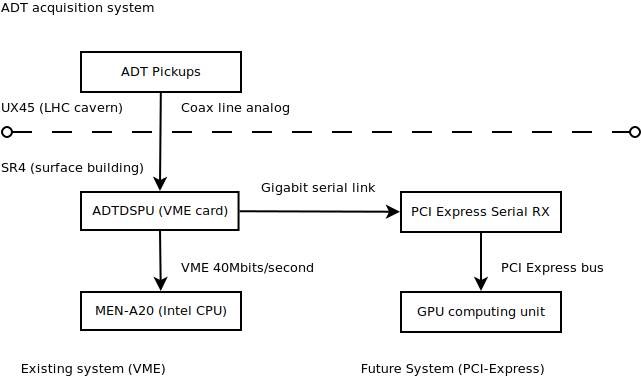
\includegraphics[scale=0.3]{acquisition.pdf}
\end{figure}

   \subsection{Estimated Bandwith}

\begin{figure}
\caption{Acquisition data flow}
\centering
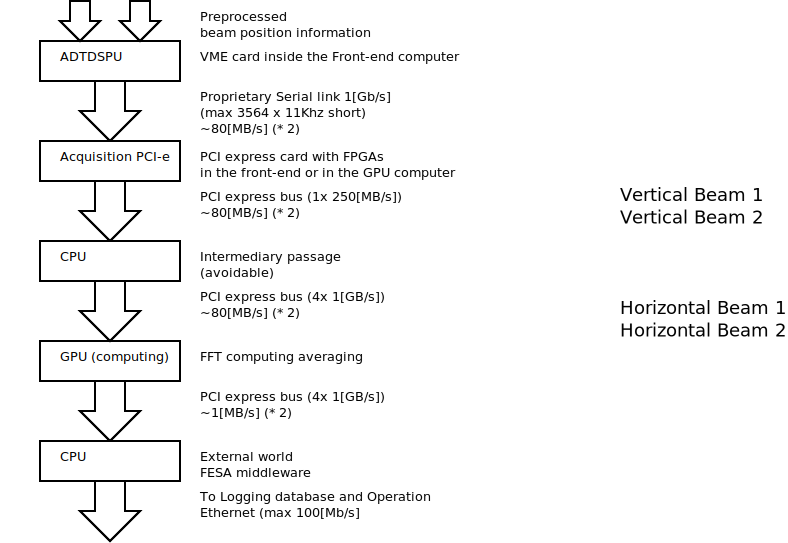
\includegraphics[scale=0.3]{dataflow.pdf}
\end{figure}

   \subsection{Software}

\section{FFT}

\section{SVD}
